\section{Auswertung}
\subsection{Zählrohr-Charakteristik}
In der Tabelle (\ref{tab:1}) sind die folgenden Messdaten aufgelistet und in
der Abbilung (\ref{abb:6}) graphisch dargestellt.
\begin{table}[H]
  \centering
  \caption{Messaufnahme zur Bestimmung des Plateaus.}
  \label{tab:1}
  \begin{tabular}{c c c c c c c c}
    \toprule
    $U \, /\, V$ & $N$ & $U \, /\, V$ & $N$ & $U \, /\, V$ & $N$ & $U \, /\, V$ &$N$ \\
    \midrule
\cellcolor{red}300 & \cellcolor{red}0 &410 & 13155 &530& 13336 &640& 13563\\
    310 & 12111 &420 & 13885 &540& 13225 &650& 13917\\
    320 & 12575 &430 & 12954 &550& 13318 &660& 13709\\
    330 & 12674 &450 & 13184 &560& 13376 &670& 13721\\
    340 & 12504 &460 & 13193 &570& 13200 &680& 13918\\
    350 & 12753 &470 & 13011 &580& 13514 &690& 13663\\
    360 & 12838 &480 & 13205 &590& 13438 &700& 14302\\
    370 & 12961 &490 & 13022 &600& 13363 &-& -\\
    380 & 12936 &500 & 13303 &610& 13288 &-& -\\
    390 & 12794 &510 & 13076 &620& 13446 &-& -\\
    400 & 13076 &520 & 13363 &630& 13495 &-& -\\
    \bottomrule
  \end{tabular}
\end{table}
\begin{figure}[H]
  \centering
  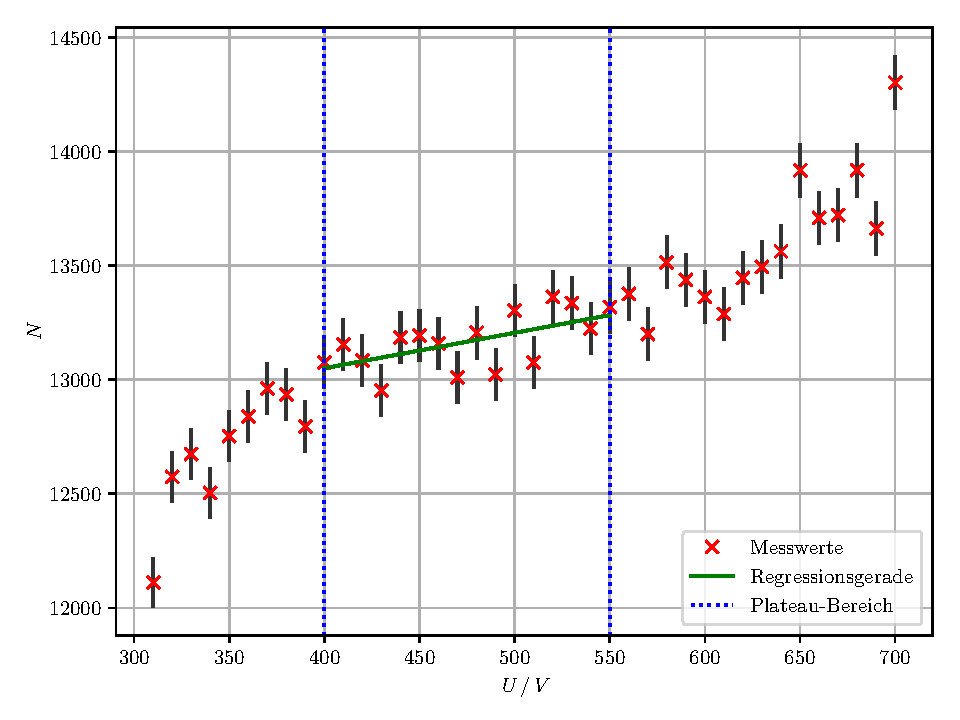
\includegraphics{plot1.pdf}
  \caption{Darstellung der Messdaten mit Fehlerbalken sowie die Einteilung des Plateaus.}
  \label{abb:6}
\end{figure}
Es ist zu beachten, dass der erste Messwert (rötlich hinterlegt) nicht in der Auswertung berücksichtig wird,
da er physikalisch nicht sinnvoll ist.
Das Plateau beginnt bei $\SI{400}{\volt}$ und endet bei $\SI{550}{\volt}$.
Für diesen Kurvenabschnitt wird eine lineare Auschgleichsrechnung mit Python 3.6 durchgeführt.
Somit ergibt sich für die Parameter der Geraden:

\begin{itemize}
  \item m = \SI{1.55(55)}{\per\volt}
  \item b = \num{12429.16(26459)}
\end{itemize}

Anschließend wird die Plateau-Steigerung in $\%$ pro $100 \, V$ mit

\begin{equation*}
  s = \frac{f(500)}{f(400)} \cdot 100 - 100 \%
\end{equation*}

bestimmt.
Die Steigerung beträgt $s = \num{1.2(4)} \%$.

\subsection{Totzeit des Zählrohrs}
Wie in der Durchführung angesprochen wurde, wird zunächst die Totzeit $T_\text{tot}$ sowie die Erhohlungszeit $T_\text{re}$ von dem Oszilloskop
abgelesen. In der Tabelle (\ref{tab:2}) sind die Messwerte dargestellt und anschließend wird der Mittelwert sowie die Standardabweichung
bestimmt.
\begin{table}[H]
  \centering
  \caption{Messdaten von der Ablesung am Oszilloskop.}
  \label{tab:2}
  \begin{tabular}{c c c}
    \toprule
    $U \, /\, V$ & $T_\text{tot} / s$ & $T_\text{re} / s$\\
    400 & 0.18 & 0.42\\
    500 & 0.2 & 0.7\\
    600 & 0.22 & 0.88\\
    \bottomrule
  \end{tabular}
\end{table}
Für den Mittelwert sowie die Standardabweichung werden die Formeln (\ref{fel:3}) und (\ref{fel:4})

\begin{equation}
    \bar{x} = \frac{1}{N} \sum_{i=1}^{N} x_i
    \label{fel:3}
\end{equation}

\begin{equation}
  \Delta \bar{x} = \frac{1}{\sqrt{N}\sqrt{N-1}} \sqrt{\sum_{i}(x_i-\bar{x})^2}
  \label{fel:4}
\end{equation}

verwendet. Es folgt für die beiden Zeiten folgende Werte:

\begin{itemize}
  \item $T_\text{tot} = \SI{0.20(1)}{\second}$
  \item $T_\text{re} = \SI{0.67(19)}{\second}$
\end{itemize}

Nun wird die Totzeit mithilfe der Zwei-Quellen-Methode bestimmt.
Die Messaufnahmen für die beiden Präperate ergeben:

\begin{itemize}
  \item $N_1 = 13100$
  \item $N_2 = 1393$
  \item $N_{1+2} = 14668$
\end{itemize}

Zur Berechnung der Totzeit wird die Formel (\ref{eq:2}) verwendet.
Da der Messwert $N_{1+2}$ größer ist als $N_1 + N_2$ bei dieser Formel eine
negative Totzeit herauskommen. Deshalb erigbt sich eine negative Totzeit, was
physikalisch nicht sinnvoll ist.
Das Ergebnis  für die Totzeit lautet somit:

\begin{equation*}
  T_{Totzeit} = (-5 \pm 5) \cdot 10^{-6} \, s
\end{equation*}


\subsection{Messung der freigesetzen Ladungsmengen}

Für die Berechnung der Ladungsmenge wird die Formel (\ref{eq:1}) umgestellt

\begin{equation*}
  \Delta Q =\overbrace{n}^{\mathclap{\text{Anzahl}}} \, \cdot \, \underbrace{e}_{\mathclap{\text{Elementarladung}}}  =  \frac{I \cdot \Delta t}{Z}
\end{equation*}

Da nur die Anzahl der Teilchen gesucht wird, wird die vorherige Gleichung noch durch die Elementarladung geteilt und in der Tabelle (\ref{tab:3})
dargestellt. Dabei ist Z fehlerbehaftet.

\begin{table}[H]
  \centering
  \caption{Messung bei $U=520 \, V$ und $\Delta t = 60 \, s$.}
  \label{tab:3}
      \begin{tabular}{c c c c c c}
        \toprule
        $U \, /\, V$ & $I \,/\, \mu A $ & $n \,/\, 10^{10} Teilchen$ &
        $U \, /\, V$ & $I \,/\, \mu A $ & $n \,/\, 10^{10} Teilchen$ \\
        \midrule
        310 & 0.1 & 0.309 \pm 0.002 & 510 & 0.6 & 1.721 \pm 0.015\\
        320 & 0.2 & 0.596 \pm 0.005 & 520 & 0.6 & 1.684 \pm 0.015\\
        330 & 0.2 & 0.591 \pm 0.005 & 530 & 0.7 & 1.968 \pm 0.017\\
        340 & 0.2 & 0.599 \pm 0.005 & 540 & 0.7 & 1.985 \pm 0.017\\
        350 & 0.2 & 0.588 \pm 0.005 & 550 & 0.8 & 2.253 \pm 0.020\\
        360 & 0.2 & 0.584 \pm 0.005 & 560 & 0.8 & 2.243 \pm 0.019\\
        370 & 0.2 & 0.579 \pm 0.005 & 570 & 0.8 & 2.273 \pm 0.020\\
        380 & 0.3 & 0.869 \pm 0.007 & 580 & 0.8 & 2.219 \pm 0.019\\
        390 & 0.3 & 0.879 \pm 0.008 & 590 & 0.8 & 2.232 \pm 0.019\\
        400 & 0.3 & 0.860 \pm 0.008 & 600 & 0.9 & 2.526 \pm 0.022\\
        410 & 0.3 & 0.855 \pm 0.007 & 610 & 0.9 & 2.539 \pm 0.022\\
        420 & 0.4 & 1.146 \pm 0.010 & 620 & 1.0 & 2.789 \pm 0.023\\
        430 & 0.4 & 1.158 \pm 0.010 & 630 & 1.0 & 2.779 \pm 0.024\\
        440 & 0.4 & 1.138 \pm 0.009 & 640 & 1.0 & 2.765 \pm 0.024\\
        450 & 0.5 & 1.421 \pm 0.012 & 650 & 1.0 & 2.695 \pm 0.023\\
        460 & 0.5 & 1.424 \pm 0.012 & 660 & 1.0 & 2.735 \pm 0.023\\
        470 & 0.5 & 1.441 \pm 0.013 & 670 & 1.1 & 3.006 \pm 0.026\\
        480 & 0.6 & 1.704 \pm 0.015 & 680 & 1.1 & 2.964 \pm 0.025\\
        490 & 0.6 & 1.728 \pm 0.015 & 690 & 1.2 & 3.294 \pm 0.028\\
        500 & 0.6 & 1.691 \pm 0.014 & 700 & 1.3 & 3.409 \pm 0.029\\
        \bottomrule
      \end{tabular}
\end{table}

\newpage
